\subsection{M.PC.AC - Actual Cost}

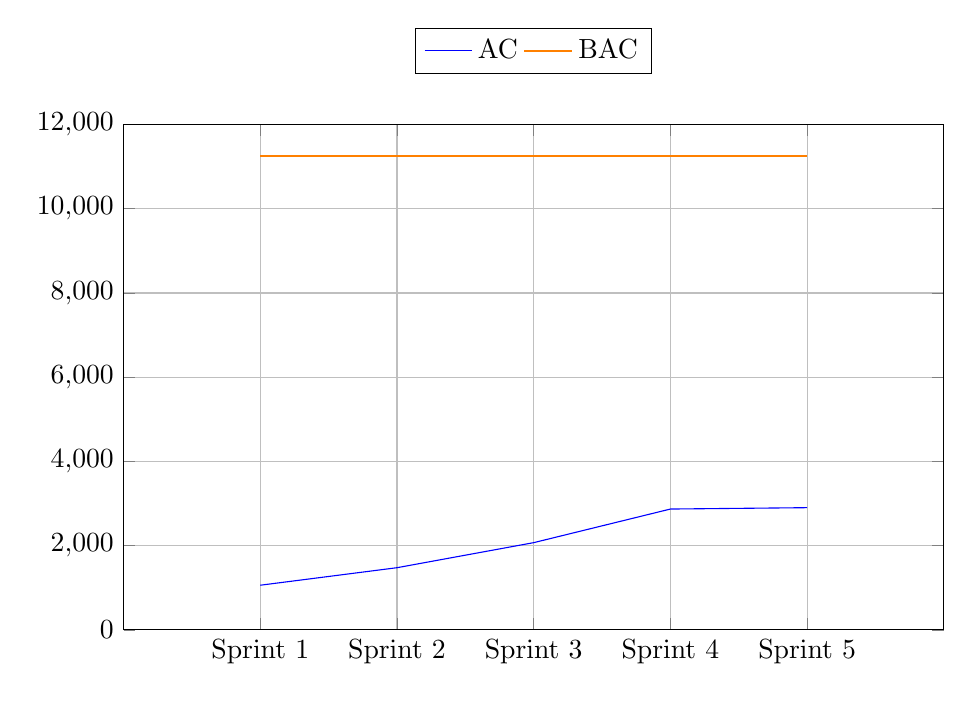
\begin{tikzpicture}
    \begin{axis}[
        width=12cm, height=8cm,
        ymin=0, ymax=12000,
        xmin=0, xmax=6,
        xtick={1, 2, 3, 4, 5},
        xticklabels={Sprint 1, Sprint 2, Sprint 3, Sprint 4, Sprint 5},
        xlabel={},
        ylabel={},
        grid=major,
        scaled ticks=false,
        legend style={at={(0.5,1.1)}, anchor=south, legend columns=-1},
    ]
    \addplot[color=blue] coordinates {(1, 1061) (2, 1477) (3, 2072) (4, 2870) (5, 2902.5)};
    \addlegendentry{AC}
    \addplot[orange, thick] coordinates {(1, 11250) (5, 11250)};
    \addlegendentry{BAC}
    \end{axis}
\end{tikzpicture}
\subsubsection{RTB}
Il grafico mostra l'incremento progressivo dei costi totali sostenuti a ogni \glossario{sprint}, 
includendo sia i costi per le attività completate sia quelli per le attività ancora in corso.